\chapter{Emscripten}
\label{cha:emscripten}

JavaScript is often called an assembly language of the Web.\cite{javascript-assembly-of-web} One could argue that since only one language is supported by browsers it could be made a compilation target similar to an assembler for CPU. This statement is flawed, since eventually JavaScript is translated to assembly making it only an intermediate step. Probably, a resemblance to ByteCode in JVM, which is a compilation target of multiple languages like Java, Scala and Clojure is more in place.
Nevertheless, recent years have shown multiple projects aimed at converting code to JavaScript. Some introduce new syntax like CoffeeScript, Dart or TypeScript, while still serving the same purpose -- providing human readable code that is interpreted in browser on the fly. Others, which are the focus of this chapter, aim to convert existing projects to run in a browser.

Several new projects are connected to make this happen. The first steps in conversion between languages were made with the LLVM project\cite{llvm} which currently is a collection of tools and compilers converting code to and from intermediate representation (LLVM IR). For C++ Clang\cite{clang} is a conversion tool.

\begin{figure}[h!]
  \caption{Pipeline of Emscripten conversion. Source: \cite{javascript-assembly-of-web}}
  \label{img:emscriptenpipeline}
  \centering
	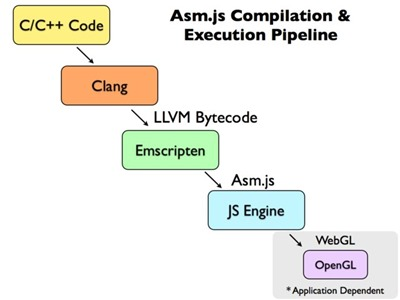
\includegraphics[width=8cm]{emscripten/pipeline.jpg}
\end{figure}

The code in LLVM is suitable for further conversion to language like JavaScript. This part is handled by the Emscripten\cite{emscripten} project. Initially, the compilation target for Emscripten was plain JavaScript. With recent developments the asm.js\cite{asmjs} library was created. It provides syntax built on top of JavaScript, which is strongly typed and easily translatable to assembly language. Asm.js details are explained in section \ref{sec:asmjsoverview}.

\lstinputlisting[caption=Example of code using asm.js,label=listing:asmjs]{emscripten/asm.js}

The project, built in cooperation with Mozilla Foundation, has its own engine for Firefox -- OdinMonkey, designed to run faster for this limited and well-defined syntax.

Altogether these projects resulted in multiple libraries and games converted from the native version to JavaScript.

Proof-of-concept demo, made in cooperation between Mozilla and Unreal, is Epic Citadel HTML5 -- Unreal Engine 3 technology demo\cite{epiccitadel}  instance running in the browser.\cite{epiccitadelhtml5} The companies claim it took only four days to complete the conversion.

\begin{figure}[h!]
  \caption{Epic Citadel screenshot}
  \label{img:epicitadel}
  \centering
	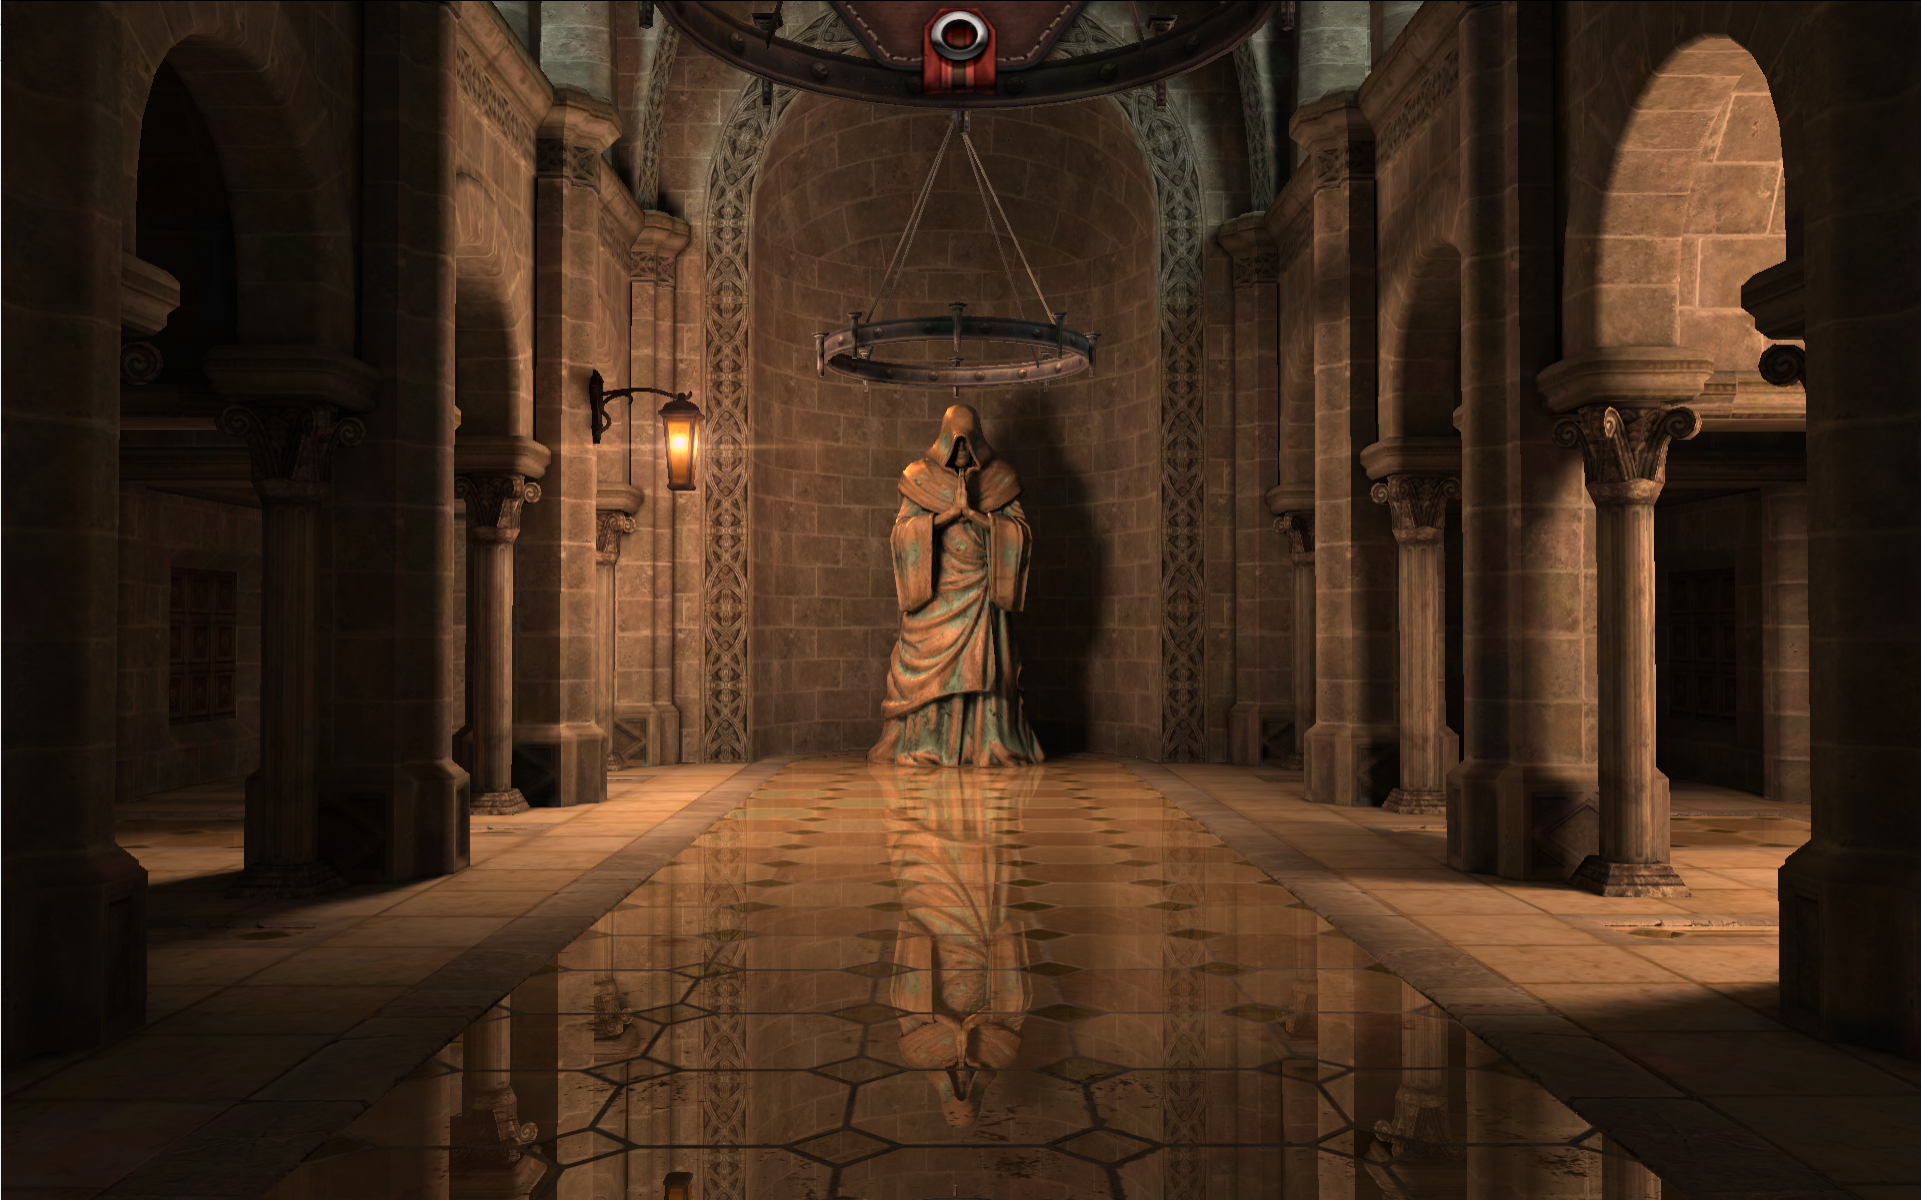
\includegraphics[width=16cm]{emscripten/epic-citadel.jpg}
\end{figure}

Another example of a successfully converted project is ammo.js\cite{ammojs} -- originating from the Bullet physics engine.

\begin{figure}[h!]
  \caption{Ammo.js demo colliding 500 boxes at 30fps, available at http://kripken.github.io/ammo.js/examples/new/ammo.html}
  \label{img:epicitadel}
  \centering
	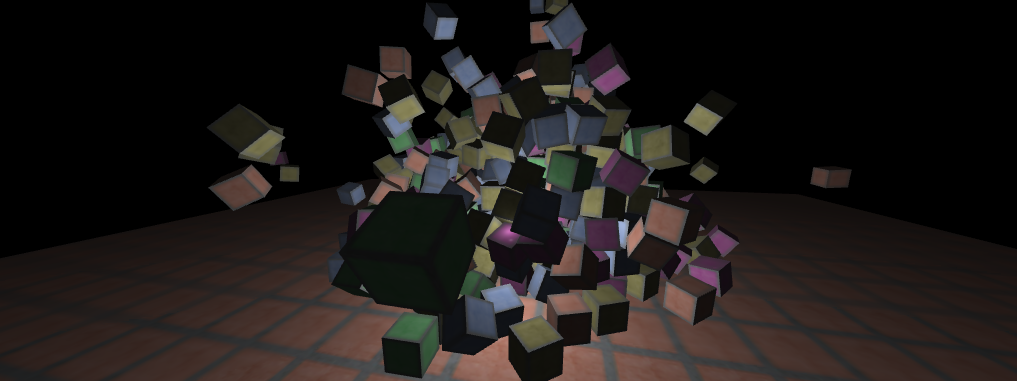
\includegraphics[width=16cm]{emscripten/ammojs.png}
\end{figure}

\section{Asm.js overview}
\label{sec:asmjsoverview}

Asm.js introduces some improvements targeted to fix performance problems of JavaScript. Ahead of time compilation enforces very specific rules on the coding style. Documentation\cite{asmjs} lists:

\subsection{Unboxed representations of integers and floating-point numbers}
\label{sec:asmjsunboxed}
In asm.js the only types allowed are integers and doubles. All numbers have annotations indicating static type (see: \ref{listing:typestree}). This way, the compiler does not have to detect possible transitions between variable types, and the overall code runs faster.

\subsection{Absence of runtime type checks}
\label{sec:asmjstypechecks}
Since asm.js works only on well-defined numbers, all function calls are monomorphic and stable. In OdinMonkey ahead-of-time compilation is able to compile them to the most optimised version without tracking method calls. In engines using JIT, methods are compiled early and newer deoptimised.

\subsection{Absence of garbage collection}
\label{sec:asmjsgc}
As shown in previous chapters, garbage collection calls are often a performance bottleneck. Asm.js solves this problem by eliminating garbage collection completely. Memory is stored in short-life variables, deallocated after the method exits and in global heaps, which are never resized or deallocated.

\subsection{Efficient heap loads and stores}
\label{sec:asmjsheap}

Heaps are global arrays of statically typed arrays, in JavaScript implemented as objects listed in \ref{table:jsarrays}. The size of the heap does not change during runtime -- it has to be calculated during the compilation and incorrect prediction or memory leaks may result in buffer overflow. Heaps are always passed as an argument to asm.js modules. Each module may reference part of the heap and use it as long as necessary.

\begin{table}[h!]
\caption{Statically typed arrays in JavaScript}
\centering
\label{table:jsarrays}
\begin{tabular}{|l|l|l|}
  	\hline
View Type & Element Size (Bytes) & Element Type \\ \hline
Uint8Array & 1 & intish \\ \hline
Int8Array & 1 & intish \\ \hline
Uint16Array & 2 & intish \\ \hline
Int16Array & 2 & intish \\ \hline
Uint32Array & 4 & intish \\ \hline
Int32Array & 4 & intish \\ \hline
Float32Array & 4 & doublish \\ \hline
Float64Array & 8 & doublish \\ \hline
\end{tabular}
\end{table}

\subsection{Summary}
\label{sec:asmjssummary}

These solutions remove some of the performance bottlenecks described in previous chapters. The code suitable to run with asm.js is almost unreadable by the programmer, and resembles an assembly code. Asm.js is not designed to be a language used by a programmer, it is mainly a target for compilation using converters like Emscripten.

Most optimisation used by asm.js is consistent with the code that is expected by V8 engine -- variables and methods are monomorphic, garbage collection is close to zero. It is worth noting that a code written by hand is almost always shorter than one generated by Emscripten. A partial solution to this is the built-in Google Closure Compiler, used on output of Emscripten and different levels of optimisation.
In tests mentioned in this paper, all solutions take 2 to 4kB compiled, while Emscripten produces over 450kB of code for each. This affects real life performance by lengthening at least transfer and parse time for code. The average parse time of 1kB of JS is believed to be up to 1ms\cite{best-practices-mobile}. The global average bandwidth was 3.1 Mbps in Q1 2013\cite{stateoftheinternet} thus transfer of each kilobyte is around 2.5ms. In total, the load time of the tested code is approximately 1.5 second on an average bandwidth and platform. In the case of larger applications and games, the load time may be significantly greater and should be taken into consideration.
